


%%++++++++++++++++++++++++++++++++++++++++++++++++++++++++++++++++++++++++++++++
%%  Packages
\usepackage[english]{babel} 			% Langue
\usepackage[utf8]{inputenc}											% Encodage
\usepackage[T1]{fontenc}											  % Requis

\usepackage[pdftex]{graphicx}										% Images 
\usepackage{fancyhdr}												% Spécifier Entête et pieds.
\usepackage[margin=2.5cm]{geometry}

\usepackage{url}													% URL 
\usepackage{hyperref}
\usepackage{verbatim}												% Texte entre 	\begin{verbatim}  \end{verbatim} ne sera pas interprété
\usepackage{listliketab}											% List spéciale, notament comme tableau
\usepackage{longtable}
\usepackage{booktabs}												% Permet de faire des tableau plus avec des traits
% Exemple:
%\begin{tabular}{llr}
%\toprule
%\multicolumn{2}{c}{Item} \\
%\cmidrule(r){1-2}
%Animal & Description & Price (\$) \\
%\midrule
%Gnat  & per gram & 13.65 \\
%      & each     &  0.01 \\
%\bottomrule
%\end{tabular}

\usepackage{color}		
%% \definecolor{orange}{RGB}{255,127,0} http://en.wikibooks.org/wiki/LaTeX/Colors

\usepackage{tabularx}											% Tableau streatching 
\usepackage{colortbl}											% Permet des tableaux exotiquement colorier 
\usepackage{wrapfig}											% Permet d'alligner une figure à guache ou à droite
%\begin{wrapfigure}{r}{40mm}
%  \begin{center}
%    \includegraphics{toucan.eps}
%  \end{center}
%  \caption{The Toucan}
%\end{wrapfigure}
\usepackage{rotating}
\usepackage{amsmath}
\usepackage{subfig}
\usepackage{pdfpages}										% inclus pdf http://www-hep2.fzu.cz/tex/texmf-dist/doc/latex/pdfpages/pdf-ex.pdf
\usepackage[subfigure]{tocloft}
%\begin{figure}[htp]
%  \begin{center}
%    \subfigure[Original image]{\label{fig:edge-a}\includegraphics[scale=0.75]{toucan.eps}}
%    \subfigure[After Laplace edge detection]{\label{fig:edge-b}\includegraphics[scale=0.75]{laplace_toucan.eps}} \\
%    \subfigure[After Sobel edge detection]{\label{fig:edge-c}\includegraphics[scale=0.75]{sobel_toucan.eps}}
%  \end{center}
%  \caption{Various edge detection algorithms}
%  \label{fig:edge}
%\end{figure}
\usepackage[table]{xcolor}								
\usepackage{url}	
%\usepackage{lscape} 								%% Texte en landspcae
%\begin{landscape}
%notre texte
%\end{landscape}

%%++++++++++++++++++++++++++++++++++++++++++++++++++++++++++++++++++++++++++++++
%%  macros
\newcommand{\todo}[1]{\colorbox{red}{\color{white}:TODO:}#1}




\usepackage{color}
\usepackage{listings}

\definecolor{colKeys}{rgb}{0,0,1} 
\definecolor{colIdentifier}{rgb}{0,0,0} 
\definecolor{colComments}{rgb}{0,0.5,1} 
\definecolor{colString}{rgb}{0.6,0.1,0.1} 

\lstset{ 
basicstyle=\ttfamily\small, % 
identifierstyle=\color{colIdentifier}, % 
keywordstyle=\color{colKeys}, % 
stringstyle=\color{colString}, % 
commentstyle=\color{colComments} 
} 
\lstset{language=java,captionpos=b} 

%%%%%%%%%%%%%%%%%%%%%%%%
%%  Design
%%%%%%%%%%%%%%%%%%%%%%%%%%
%%
%%  Pren1 Schlussdokument
%%  Kopf und Fusszeilen
%%  CT
%%
%%%%%%%%%%%%%%%%%%%%%%%%

\pagestyle{fancy}
  \renewcommand\headrulewidth{0.4pt}
  \fancyhf{}
  \setlength{\headheight}{35.60004pt}
%  \addtolength{\texthight}{-2*\headheight}
  \lhead{
    \protect
\includegraphics[height=32pt]{./images/model/eifr-logo.jpg}
  }
  \rhead{
    Mobile development TD3\\
   Jonathan Stoppani et Elias Medawar\\
  }
  \cfoot{
    \thepage
  }
\fancypagestyle{plain}{
  \renewcommand\headrulewidth{0.4pt}
  \fancyhf{}
  %\addtolength{\headheight}{\baselineskip}
  \lhead{
    \protect
\includegraphics[height=32pt]{./images/model/eifr-logo.jpg}
  }
  \rhead{
    Mobile development TD3\\
     Jonathan Stoppani et Elias Medawar\\
  }
  \cfoot{
  }
}
\fancypagestyle{empty}{
  \renewcommand\headrulewidth{0pt}
  \fancyhf{}
  %\addtolength{\headheight}{\baselineskip}
  \lhead{
  }
  \cfoot{
  }
}

\begin{document}
	\begin{titlepage}
	
	%\sffamily

		
	\addtolength{\leftskip}{-1cm}\addtolength{\rightskip}{-3.5cm}
	%\sffamily
	\vfill
	
	\hspace{0.10cm}	
\includegraphics{./images/model/eifr-logo.jpg} 

	\vfill
	\hspace{8.99cm}\Huge Mobile development  3 
	
	\hspace{9.08cm}\LARGE Report TD 3 : 
	      
	\vfill
	\Large
	
	\hspace{9.08cm}  Jonathan Stoppani et Elias Medawar
	
	\vfill
	\hspace{9.08cm}\normalsize Version:  \today
	\vfill
	\thispagestyle{empty}
	\clearpage

\end{titlepage}

	
	%%%%%%%%%%%%%%%%%%%%%%%%
%%
%%  Pren1 Schlussdokument
%%  Kopf und Fusszeilen
%%  CT
%%
%%%%%%%%%%%%%%%%%%%%%%%%

\pagestyle{fancy}
  \renewcommand\headrulewidth{0.4pt}
  \fancyhf{}
  \setlength{\headheight}{35.60004pt}
%  \addtolength{\texthight}{-2*\headheight}
  \lhead{
    \protect
\includegraphics[height=32pt]{./images/model/eifr-logo.jpg}
  }
  \rhead{
    Mobile development TD3\\
   Jonathan Stoppani et Elias Medawar\\
  }
  \cfoot{
    \thepage
  }
\fancypagestyle{plain}{
  \renewcommand\headrulewidth{0.4pt}
  \fancyhf{}
  %\addtolength{\headheight}{\baselineskip}
  \lhead{
    \protect
\includegraphics[height=32pt]{./images/model/eifr-logo.jpg}
  }
  \rhead{
    Mobile development TD3\\
     Jonathan Stoppani et Elias Medawar\\
  }
  \cfoot{
  }
}
\fancypagestyle{empty}{
  \renewcommand\headrulewidth{0pt}
  \fancyhf{}
  %\addtolength{\headheight}{\baselineskip}
  \lhead{
  }
  \cfoot{
  }
}
	
	\section{Exercice : 1}
		\subsection{Activité avec changements d'états}
		
		\begin{center}
			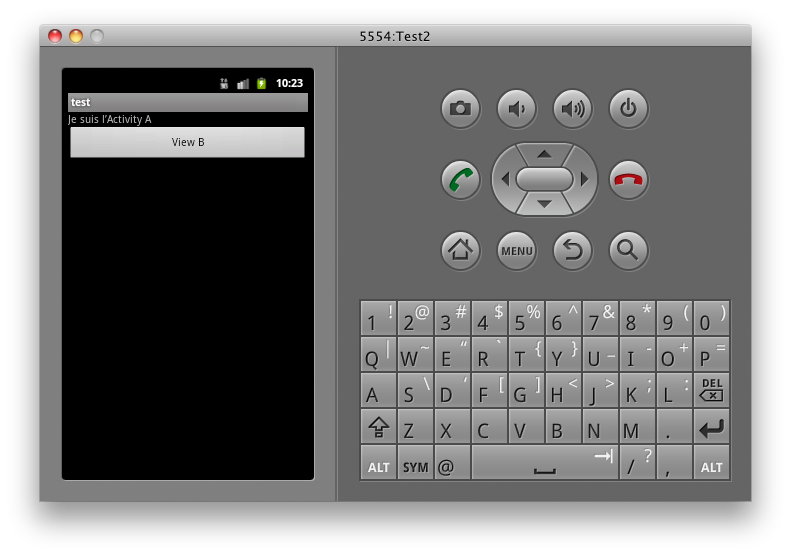
\includegraphics[width=1\textwidth]{./images/ex1a.png}
			Une activité basique avec un texte et un bouton
		\end{center}		
		
		\begin{center}
			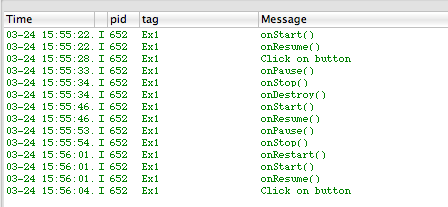
\includegraphics[width=1\textwidth]{./images/ex1.png}
			Le résultat des différents passages d'états.
		\end{center}		
		\subsection{ActivityA avec changements d'états}
		
		\begin{center}
			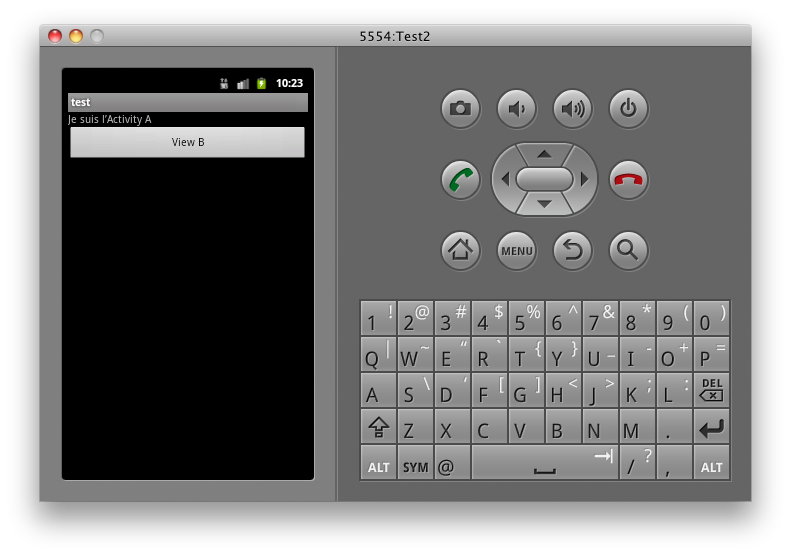
\includegraphics[width=1\textwidth]{./images/ex1a.png}
			Une activité basique avec un texte et un bouton
		\end{center}		
		
		\begin{center}
			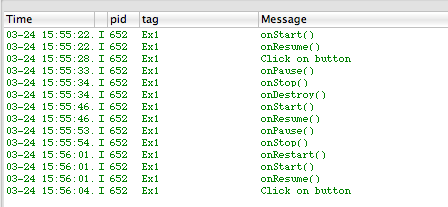
\includegraphics[width=1\textwidth]{./images/ex1.png}
			Le résultat des différents passages d'états.
		\end{center}	
		\subsection{ActivityB depuis activityA}
\lstset{language=java,captionpos=b,caption={Code pour capturer l'envement du click sur le bouton}} 
\begin{lstlisting}
protected void onCreate(Bundle savedInstanceState) {
  super.onCreate(savedInstanceState);
  setContentView(R.layout.main);
  Button b = (Button)findViewById(R.id.btnCreateView);
  b.setOnClickListener(new OnClickListener() {
    @Override
    public void onClick(View v) {
      Log.i("Ex1","Click on button");
      Intent intent = new Intent(getApplicationContext(),ActivityB.class);
      startActivity(intent);
    }
  });
}
\end{lstlisting}

\lstset{language=java,captionpos=b,caption={Code de l'activityB}} 
\begin{lstlisting}
public class ActivityB extends Activity {
  @Override
  protected void onCreate(Bundle savedInstanceState) {
    setContentView(R.layout.activity);
    super.onCreate(savedInstanceState);
  }
}
\end{lstlisting}



	\section{Exercice : 2}
	Le code source des interfaces graphique ainsi que des actions étant déjà fournit dans l'exercice, il ne sera pas insérer dans le rapport. Néanmoins il est disponible sur gitHub à l'adresse: https://github.com/eia-fr/mobileDev/tree/master/TD5
	\subsection{Standard}
	\begin{enumerate}
	\item Dès le clic sur le bouton, un erreur se produit et l'application se termine. Ce résultat n'est pas étonnant vu qu'on a pas encore déployer(installer) l'application 2. En dehors de cela les bons écrans sont affiché. 
		\begin{figure}[!h]
				\centering
				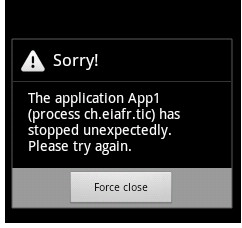
\includegraphics[scale=0.5]{./images/error2Notexist.png}
				\caption{Erreur application non existante}
		\end{figure}
		\item Les écrans sont affichés dans le bon ordre(Activity 1 - 2 -3 - A) et sans problème.			
			Dans la données il n'était pas indiqué que dans le ficher \textit{AndroidManifest.xml} \ref{AndroidManifestApp1}  de l'application 1 l'activityA devait répondre au filtre depuis une autre application(comme pour l'activity2). Nous avons conclus que c'était un oubli et avons tout de même insérer le code\ref{AndroidManifestApp1}  qui nous de faire permet cet opération. Nous ne sommes pas encore capable d'expliquer exactement ce code mais ceci sera traité dans la prochaine leçon.
			
\lstset{language=XML,numbers=left, numberstyle=\tiny,captionpos=b,caption={Fichier AndroidManifest de l'application 1 avec un filtre(ligne 14 à 16) permetant l'accés à l'activityA depuis une autre application} , label=AndroidManifestApp1} 
			\begin{lstlisting}
<?xml version="1.0" encoding="utf-8"?>
<manifest xmlns:android="http://schemas.android.com/apk/res/android"
      package="ch.eiafr.tic.application1"
      android:versionCode="1"
      android:versionName="1.0">
      
    <application android:icon="@drawable/icon" android:label="Application1">
        <activity android:name=".ActivityA"
                  android:label="@string/app_name">
            <intent-filter>
                <action android:name="android.intent.action.MAIN" />
                <category android:name="android.intent.category.LAUNCHER" />
            </intent-filter>
            <intent-filter>
                <action android:name="ch.eiafr.tic.application1.VIEW_ACTIVITYA" />
                <category android:name="android.intent.category.DEFAULT" />
            </intent-filter>
        </activity>
        <activity android:name=".ActivityB"
                  android:label="@string/app_name">
        </activity>
    </application>
</manifest>
}
\end{lstlisting}

\item Refaire le point 1. \\
Les fenêtre s'affiche dans le bon ordre et sans aucune erreur. Ceci semble logique, vu que l'on a désormais les 2 applications qui sont désormais installé. 
	\end{enumerate}


	\subsection{SingleTask}
			\begin{enumerate}
			\item Démarrer l'Activity1 (via un clique sur son icône), affiche l'activity1
			\item Cliquer sur le bouton de l’Activity1, affiche l'activity2
			\item Cliquer sur le bouton de l’Activity2, affiche l'activity3
			\item Cliquer sur le bouton HOME, affiche la page principale du système.
			\item Démarrer l'ActivityA (via un clique sur son icône), affiche l'activityA
			\item Cliquer sur le bouton de l’ActivityA, affiche l'activity B.
			\item  Cliquer sur le bouton de l’ActivityB, affiche l'activity2
			\item Cliquer sur le bouton BACK,affiche l'activityB
			\item Cliquer sur le bouton BACK,affiche l'activityA
			\item Cliquer sur le bouton BACK, affiche la fenêtre de sélection(lancement) d'application.
			\item Démarrer l'Activity1 (via un clique sur son icône),affiche l'actvity 3.
			\item Cliquer sur le bouton BACK, affiche l'activity 2
			\item Cliquer sur le bouton BACK , affiche l'activity 1
			\item Cliquer sur le bouton BACK , affiche la fenêtre de sélection(lancement) d'application.
			\end{enumerate}
			
\textbf{Modification Activity2 en Single Task}
\lstset{language=XML,numbers=left, numberstyle=\tiny,captionpos=b,caption={Modification dans le fichier manifest pour mettre l'activity2 accésible en mode singleTask} , label=changeActivity2mode} 
\begin{lstlisting}
<activity android:name="Activity2"
                  android:label="@string/app_name"
                  android:launchMode="singleTask">
           <intent-filter>
            <action android:name="ch.eiafr.tic.application2.VIEW_ACTIVITY2"/> 
            <category android:name="android.intent.category.DEFAULT"/>
          </intent-filter> 
</activity>
\end{lstlisting}
			\begin{enumerate}
					\item Démarrer l'Activity1 (via un clique sur son icône), affiche l'activity1
					\item Cliquer sur le bouton de l’Activity1, affiche l'activity2
					\item Cliquer sur le bouton de l’Activity2, affiche l'activity3
					\item Cliquer sur le bouton HOME, affiche la page principale du système.
					\item Démarrer l'ActivityA (via un clique sur son icône), affiche l'activityA
					\item Cliquer sur le bouton de l’ActivityA, affiche l'activity B.
					\item  Cliquer sur le bouton de l’ActivityB, affiche l'activity2
					\item Cliquer sur le bouton BACK,affiche l'activity1
					\item Cliquer sur le bouton BACK,affiche l'activityB
					\item Cliquer sur le bouton BACK,affiche l'activityA
					\item Cliquer sur le bouton BACK , affiche la fenêtre de sélection(lancement) d'application.
					\item Démarrer l'Activity1 (via un clique sur son icône),affiche l'actvity 1.
			\end{enumerate}
			Le changement commence à l'étape 8 quand on clique BACK, l'activity1 sera affiché au lieu de l'activityB est une fois les activity de la tache courante terminé, on reprendra à au sommet de la pile de la tache précédente. Ceci est dû à la spécification du mode singleTask. Explication trouvé dans les slides du cours à la page 11.
			
\subsection{SingleInstance}
			\begin{enumerate}
					\item Démarrer l'Activity1 (via un clique sur son icône), affiche l'activity1
					\item Cliquer sur le bouton de l’Activity1, affiche l'activity2
					\item Cliquer sur le bouton de l’Activity2, affiche l'activity3
					\item Cliquer sur le bouton BACK, affiche l'activity1
					\item Cliquer sur le bouton BACK, affiche l'activity2
					\item Cliquer sur le bouton BACK, affiche la fenêtre de sélection(lancement) d'application.
					\item Cliquer sur le bouton BACK, affiche la page principale du système.
			\end{enumerate}
			Deuxième séquence
			\begin{enumerate}
					\item Démarrer l'ActivityA (via un clique sur son icône), affiche l'activityA
					\item Cliquer sur le bouton de l’ActivityA, affiche l'activity B.
					\item  Cliquer sur le bouton de l’ActivityB, affiche l'activity2
					\item Cliquer sur le bouton de l'Activity affiché, affiche l'activity3
					\item Cliquer sur le bouton HOME, affiche la page principale du système.
					\item Démarrer l'Activity1 (via un clique sur son icône), affiche l'activity3
					\item Cliquer sur le bouton BACK, affiche la fenêtre de sélection(lancement) d'application.
					\item Démarrer l'ActivityA (via un clique sur son icône), affiche l'activityB
					\item Cliquer sur le bouton BACK, affiche l'activityA
					\item Cliquer sur le bouton BACK, affiche la fenêtre de sélection(lancement) d'application.
			\end{enumerate}
			

			Il existe qu'une activity par tasks c'est pour cela qu'au point 7 on reviendra pas à l'activity 2 mais au menu de sélection d'application.( http://developer.android.com/guide/topics/fundamentals/tasks-and-back-stack.html)


			\subsubsection{Questions}
			\textbf{A quoi doit t’on faire attention si l’Activity est une activity singleInstance ? } Quand on redémarre une application (exemple point 6 de la dernière séquence) l'historique de la navigation n'est pas garder. En effet on garde la task avec juste une activity et donc les autres activity ne seront plus mémorisé.
			
			\textbf{Pourquoi doit on s’assurer que les 2 applications ne soient pas déjà démarrer avant d’effectuer les séquences?} Si elles étaient déjà démarrer, on  verrait au démarrage la dernière activity visité et non la première de l'application.

	\subsection{SingleTop}
	\lstset{language=JAVA,numbers=left, numberstyle=\tiny,captionpos=b,caption={Modification faites dans la classe ActivityB pour ouvrir l'activityB quand on presse le bouton} , label=changeActivityB} 
	\begin{lstlisting}
public class ActivityB extends Activity {
 @Override
 protected void onCreate(Bundle savedInstanceState) {
  setContentView(R.layout.activityb);
  super.onCreate(savedInstanceState);
  Button b = (Button)findViewById(R.id.Bto2);
  b.setOnClickListener(new OnClickListener() {
   @Override
   public void onClick(View v) {
    Log.i("Ex2","Click on button Bto2");
    Intent intent = new Intent(getApplicationContext(),ActivityB.class);
    startActivity(intent);
   }
  });
 }
}
	\end{lstlisting}
	\begin{enumerate}
			\item Démarrer l'ActivityA (via un clique sur son icône), affiche l'activityA
			\item Cliquer sur le bouton de l’ActivityA, affiche l'activity B.
			\item  Cliquer sur le bouton de l’ActivityB, affiche l'activityB
			\item Cliquer sur le bouton BACK, affiche l'activityB.
			\item Cliquer sur le bouton BACK, affiche l'activityA.
			\item Cliquer sur le bouton BACK, affiche la fenêtre de sélection(lancement) d'application.
	\end{enumerate}
\lstset{language=XML,numbers=left, numberstyle=\tiny,captionpos=b,caption={Modification dans le fichier manifest pour mettre l'activityB  en mode singleTop} , label=changeActivity2mode} 
\begin{lstlisting}
<activity android:name=".ActivityB"
    android:label="@string/app_name" 
    android:launchMode="singleTop">
</activity>
\end{lstlisting}

	\begin{enumerate}
			\item Démarrer l'ActivityA (via un clique sur son icône), affiche l'activityA
			\item Cliquer sur le bouton de l’ActivityA, affiche l'activity B.
			\item  Cliquer sur le bouton de l’ActivityB, ne change pas d'activity
			\item Cliquer sur le bouton BACK, affiche l'activityA.
			\item Cliquer sur le bouton BACK, affiche la fenêtre de sélection(lancement) d'application.
			\item Cliquer sur le bouton BACK, affiche la page principale du système.
	\end{enumerate}
	
	Avec le mode singleTop, l'activityB ne sera pas crée plus d'une fois. 
	
	\vspace{1cm}
	\textbf{Toute les sources sont téléchargeable et accessible sur: }\\
	      https://github.com/eia-fr/mobileDev/tree/master/TD5 
\end{document}